
\section{Simulation details \label{Appendix:simulation}}

World size is directly proportional to the agent and food area. The agent
size is $[W_{r},H_{r}]=2.50 U \cdot 2U$ with an area $A_{agent}=5 U^{2}$, where U is the unit of measure used in the simulations.
Food sources are regular polygons composed by $e_{food}=32$ edges with an apothem of $ap_{food}=3 U$ corresponding to an area of
\begin{equation}
A_{food}=ap_{food}^2 \cdot e_{food} \cdot tan(\frac{\pi}{e_{food}})=28.36 U^2.
\end{equation}

It means that only $N_{max,food}=9$ robots can lie on the food disk boundary, because
\begin{equation}
A_{max,agents}=\frac{S^{2} \cdot e_{food}}{4 \cdot tan(\frac{\pi}{N_{max,food}})}=24.73 U^{2}
\end{equation}
where $S=2.0 U$. The area of the world is proportional to the areas of agents and food disks, and on their numbers.
\begin{equation}
A_{world}=(K_{1} \cdot A_{food} \cdot M) + (K_{2} \cdot A_{agent} \cdot N) + (K_{2} \cdot A_{agent} \cdot N)
\end{equation}

where $K_{o}=50,K_{a}=60$. The world is a square with a side of $L=\sqrt[2]{A_{world}}$.
The robot boundary surface is delimeted by the following points: $<-1.25,-1>,<1.25,-1>,<1.25,1>,<-1.25,1>$

Robot parameters:
\begin{itemize}
\item differential 2 wheeled driving system
\item 2 infrared sensors: placed in front of the robot, one left one right,
oriented with $\alpha(l,r)=\pm45\degree$, an aperture of $IR_{field}=30\degree$ ,
a range of $range_{IR,reflex}=2.5 U$ and $ray=3$.

\item 2 infrared sensors: placed in the back of the robot, one left one right,
oriented with $\alpha(l,r)=\pm160\degree$, an aperture of $IR_{field}=60\degree$ ,
 a range of $range_{IR,reflex}=2.5 U$ and $ray=3$.

\item 2 circular RGB cameras $ccam_{i,proximal}$ with a visibility range of
$10.0 U$: placed in front of the robot, one left one right, $h=2.0 U$
from the ground, oriented with $\alpha=\pm30\degree$, an aperture of
$field_{proximal}=60\degree$  and a resolution of $ccam_{res}=16$ pixels.
\item 2 circular RGB camers $ccam_{i,reflex}$ with a visibility range of
$8.0 U$: placed in front of the robot, one left one right,
oriented with with $\alpha=\pm30\degree$, aperture of $field_{proximal}=60\degree$
and a resolution of $ccam_{res}=16$ pixels.
\end{itemize}


Sensors' and actuators' response functions are modeled on the Alice robot by
EPFL\footnote{Ecole Polytechinique Fèdèrale de Lausanne} into the ENKI simulator environment.
Motors have a normalised speed of $[v_{min},v_{max}]=[-1,1] $ within an inversely
proportional motor noise to the speeds in $[-1,1] $, the noise is of the order
of $\pm 5\%$ for the maximum speed, for $\pm \frac{3 U}{t}$ it is $\pm 10\%$
The objects in the world have different colours that represent their type.
The agent can see colors using their RGB circular cameras.
A color is represent by 3 components: red,blue and green as a triplet $<r,g,b>$
where $r,g,b \subset [0.0,1.0]$. For example red is represented by $<1.0,0.0,0.0>$.
The rule for the colors are:
\begin{itemize}
 \item the agent's color is:$color(agent)$ $=$ $<1.0,0.0,H_{sated}(t)>$ as described in eq.\ref{eq:satstate}.
Thus an agent has a fixed red component and a blue component that expresses its internal state of satedness.
\item the food place's colour for the unlimited case is:$color(food_{infinite})$ $=$ $<0.0,1.0,0.0>$
\item the food place's colour for the limited case is:$color(food_{finite})$ $=<0.0,1.0,q(t)>$ as in eq.\ref{eq:qfood}.
\item an object with green component is a food source.
\end{itemize}

According to the ICO terminology the agent's configuration is:
\begin{itemize}
\item left and right infrared sensors are the reflex for obstacles:
world's walls, other agents, food sources
\item left and right long range camera filtering the red component
are the proximal for obstacles: other red agents, or food sources before learning
\item left and right long range camera filtering the blue component
are the distal signals for agent attraction: other agents consuming food.
\item left and right short range camera filtering the blue component
are the proximal signals for agent attraction: other agents consuming food.
\item left and right long range camera filtering the green component
are the distal signal for food attraction.
\item left and right short range camera filtering the green component
are the proximal signal for food attraction.

\end{itemize}
The back left and right infrared sensors are useful when the robot is going
backwards and bumps into an obstacle: in that case the speed is inverted.
The left,right camera inputs must be transformed from a vectorial format
to a scalar one for the input synapses. Every circular camera produces a
matrix $Vcam_{NPIXELS,3}$ where $npixels=16$, the scalar filtered input
is computed as:
\begin{equation}
vcam=\sum_{i=1}^{npixels} Vcam_{i,fcol}
\label{eq:cfilter}
\end{equation}
where $fcol$ is the chosen color component to be filtered.\\
The ICO network topology is described step by step, adding the relative features:
obstacles avoidance first, food attraction and then agent with food attraction.
Tthe configuration used for the network parameters follows.
\subsection{Obstacle avoidance}
The obstacles have a red component therefore in eq. \ref{eq:cfilter} $fcol=0$.
The agent must avoid obstacles: it means that the left input is connected with
the right output with a negative weight, and the left input is connected with
the left output with a negative weight. In this way when an obstacle is on
the left side the robot will go back turning left.
\begin{itemize}
 \item IR sensors: $W_{proximal,L}=-0.9$,$W_{proximal,R}=-1.0$
 \item short range camera: $W_{distal,L}=4.0$,$W_{distal,R}=-4.2$
 \item Filter parameters: $F_{proximal}=0.5$,$F_{distal}=0.6$,\\ $Q_{proximal}=\sqrt(2)$,$Q_{distal}=\sqrt(2)$
 Q is chosen to have a maximum flat response
\end{itemize}

\subsection{Food attraction parameters}
The food sources have a green component therefore in eq.\ref{eq:cfilter} $fcol=1$.
The agent must approach the food, therefore the left and right synaptic input
values must be equal: it means that the difference between the left and
right input must be 0.
\begin{itemize}
 \item $W_{proximal,L}=2.6$,$W_{proximal,R}=-2.8$
 \item $W_{distal,L}=3.0$,$W_{distal,R}=-3.2$
 \item Filter parameters: $F_{proximal}=0.6$,$F_{distal}=0.6$,\\$Q_{reflex}=\sqrt(2)$,$Q_{proximal}=\sqrt(2)$
\end{itemize}

\subsection{Agent with food attraction parameters}
The agents have a red and blue component therefore in eq.\ref{eq:cfilter} $fcol=0,2$.
The agent must approach the other agent, therefore the left and right synaptic
input values must be equal: it means that the difference between the left
and right input must be 0.
\begin{itemize}
 \item $W_{proximal,L}=3.0$,$W_{proximal,R}=-3.2$
 \item $W_{distal,L}=3.0$,$W_{distal,R}=-3.2$
 \item Filter parameters: $F_{proximal}=0.6$,$F_{distal}=0.6$,\\$Q_{reflex}=\sqrt(2)$,$Q_{proximal}=\sqrt(2)$
\end{itemize}

\subsection{Hysteresys effect \label{Appendix:HysteresysValue}}
If an agent is in proximity of an acute angle (it could be an angle of the
scenario or a particular spatial agent configuration) without the hysteresys
it will starve turning left and right, within the hysteresys the responses will
be delayed so it will turn first left and after some time right.
The weight connections are asymmetric to balance the outputs (using the same
weights makes the robot run in circular pathways).
Parameters are:
\begin{itemize}
 \item $W_{self,L}=0.4$,$W_{self,R}=0.4$
 \item $W_{left,right}=-0.42$,$W_{right,left}=-0.3$
\end{itemize}
The bias for the network is: $bias=2.4$.
\subsection{Physical engine and kinematic model}
Every object in the world has the following physical properties:
\begin{enumerate}
\item position is 2 dimensional vector
\item height: the height of the object, used for interaction with robot's sensors.
\item angle: the orientation of the object in the world, standard trigonometric
\item vector speed: The speed of the object
\item angle:  the orientation of the object in the world, standard trigonometric orientation.
\item angular speed: the rotation speed of the object, standard trigonometric orientation.
\item mass: the mass of the object. If below zero, the object can't move (infinite mass).
\item static friction threshold: the static friction threshold of the object.
If a force is smaller than it, the object will not move
\item viscous friction tau: the viscous friction time constant.
Half-life of speed when object is free. If lower than timestep, speed is forced to zero.
\item viscousMomentFrictionTau: the viscous friction moment time constant.
Half-life of angular speed when object is free. If lower than timestep, angular speed is forced to zero.
\item collisionAngularFrictionFactor: upon collision with static objects.
The amount of rotation transmitted to the moving object. If zero, moving object slides over static one. If one, moving object is fully rotated.
\end{enumerate}

The function that updates the state of the object is:
\small{
\begin{lstlisting}
void PhysicalObject::step(double dt)
{
	pos += speed * dt;
	angle += angSpeed * dt;
	angle = normalizeAngle(angle);
	// TODO : optimise this using ExpDecay from external math lib !
	if (viscousFrictionTau < dt)
	{
		speed = 0.0;
	}
	else
	{
		double factor = (viscousFrictionTau - dt * 0.5) /
				(viscousFrictionTau + dt * 0.5);
		speed *= factor;	
	}
	if (viscousMomentFrictionTau < dt)
	{
		angSpeed = 0;
	}
	else
	{
		//std::cerr << "0  f:" << angSpeed << std::endl;
		double factor = (viscousMomentFrictionTau - dt * 0.5) /
		(viscousMomentFrictionTau + dt * 0.5);
		angSpeed *= factor;
		//std::cerr << "angSpeed:" << angSpeed << std::endl;
		//std::cerr << "factor:" << factor << std::endl;
	}
}
\end{lstlisting}
}

The kinematic model used for the differential driving system is fairly simple:
\small{
\begin{lstlisting}
void Alice::step(double dt)
{
	double realLeftSpeed, realRightSpeed;
		
	// applied inversely proportional motor noise 

	realLeftSpeed = 1 * leftSpeed * (0.95 + random.getRange(0.05));

	// same as above
	realRightSpeed = 1 * rightSpeed * (0.95 + random.getRange(0.05));

	// forward component
	double forwardSpeed = (realLeftSpeed+realRightSpeed) / 2;
	double wheelDist = 1.9;
	// Khepera code:
	speed = Vector(
	forwardSpeed * cos(angle + angSpeed * dt * 0.5),
	forwardSpeed * sin(angle + angSpeed * dt * 0.5));
	// angle
	angSpeed += (-realLeftSpeed+realRightSpeed) / wheelDist;	
\end{lstlisting}
}

For collision detection and collision interaction, detailed information
is provided in the source code.

\subsection{Simplified social simulator \label{Appendix:simplesocialsim}}

There are $N=2,4$ and $M=2$ food sources.
The agent's area $A_{agent}=5 U^{2}$, where U is the unit of measure used in the simulations.
Food source's area $A_{food}=28.36 U^2$.
The area of the world is proportional to the areas of agents and food disks, and on their numbers.
\begin{equation}
A_{world}=(K_{1} \cdot A_{food} \cdot M) + (K_{2} \cdot A_{agent} \cdot N) + (K_{2} \cdot A_{agent} \cdot N)
\end{equation}
where $K_{o}=50,K_{a}=60$. The world is a square with a side of $L=\sqrt[2]{A_{world}}$.
For $N=2$ and $M=2$: $A_{world}=3436 U^2$ and $L=58.617$.

\subsection{Screenshots}
In figures \ref{fig:screen1},\ref{fig:screen2} there are some screenshots of
the simulator environment: the graphic interface makes use of the OpenGL API
to draw the scene.

\begin{figure}[htb]
\begin{centering}
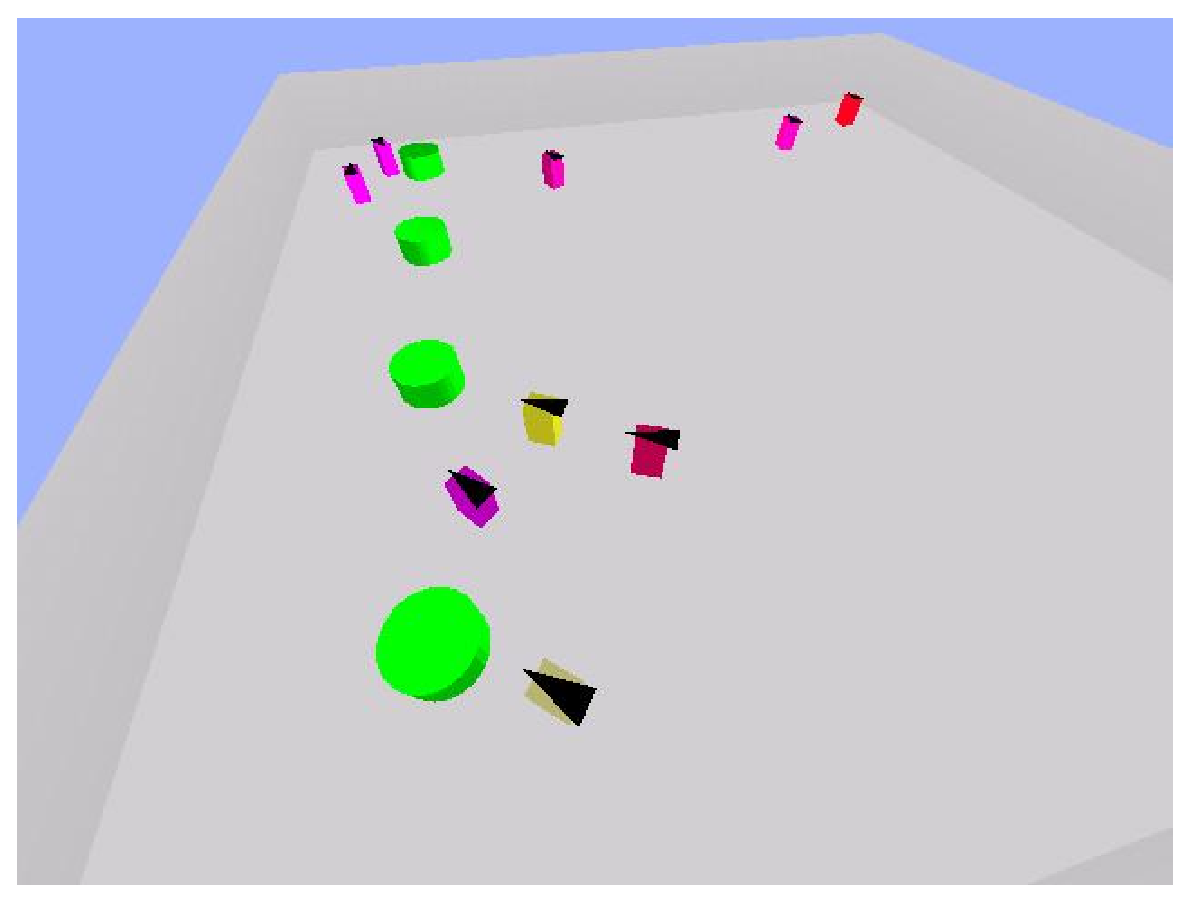
\includegraphics[scale=0.36]{socialadapt/simulator/begin.eps}
\small{
\caption[Software simulation in Enki A]{A simulation with 10 agents and 4 food disks.Yellow agents signals the
food presence, violet agents are sated, red agents are starving.
Food disks are the green disks. \label{fig:screen1}}
}
\end{centering}
\end{figure}

\begin{figure}[htb]
\begin{centering}
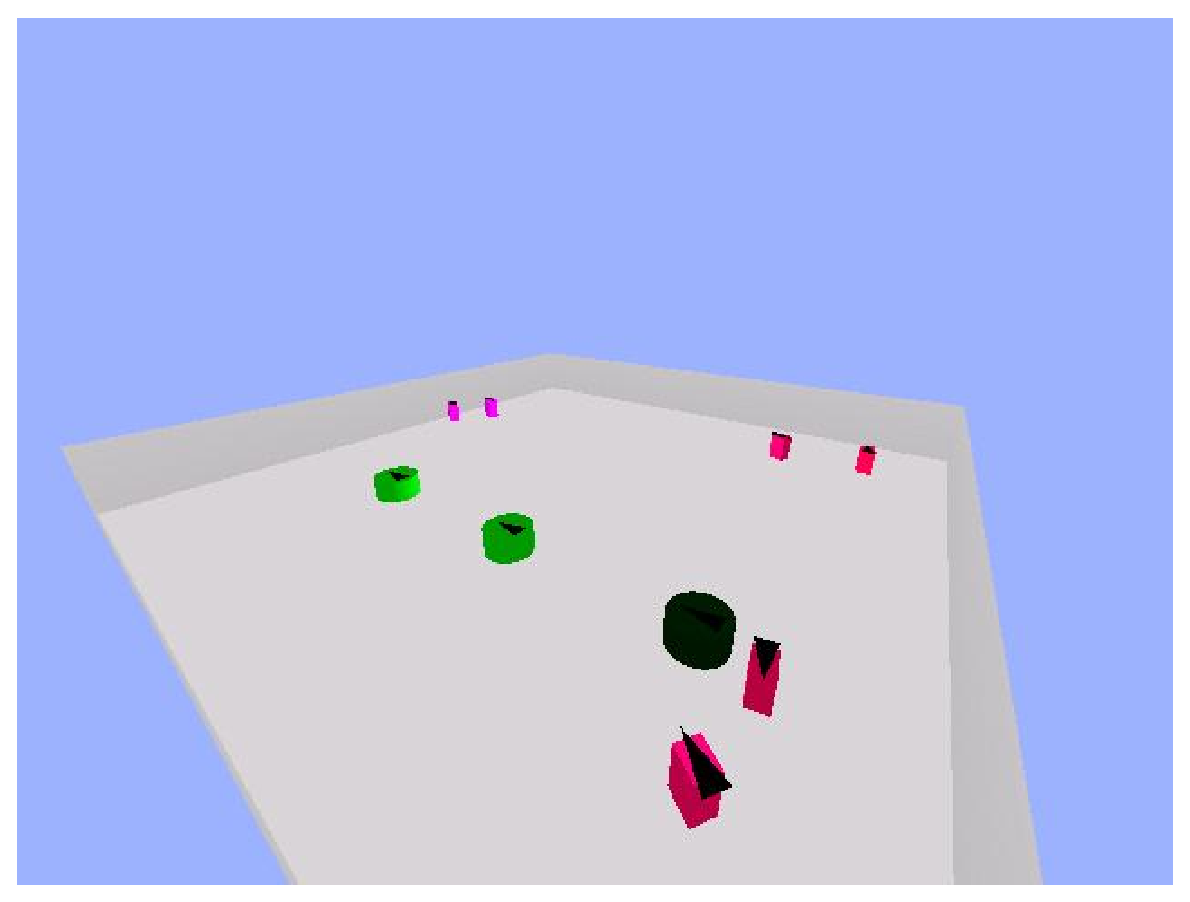
\includegraphics[scale=0.36]{socialadapt/simulator/limited.eps}
\small{
\caption[Software simulation in Enki B]{A simulation with 10 agents and 4 food disks.Yellow agents signals the
food presence, violet agents are sated, red agents are starving.
Food disks are the green disks, when the food disk is exhausted tit urns black
and agents are not attracted. \label{fig:screen2}}
}
\end{centering}
\end{figure}

\subsection{Simulation details for information flow \label{Appendix:InfoFlowSimDetails}}

The world is a toroidal square of 300x300 units ($Um$), the agent has a diameter of 10 $Um$,
the reflex antennas have a range of 40 $Um$, the predictor antennas have a range of 60 $Um$,
every food disk has a diameter of 20 $Um$, the agent consumes food after $30$ time steps.
Every food disk starts with 100 food units and, if depleted, is reset after 5 time steps.
To compute the entropy, the input space is discretised into 4 equally spaced bins
and normalised in the range [-1,1]
both for the predictor $U_1$ and the reflex $U_0$ signal, the output signal $Z$
is discretised in 8 directions.

\subsection{Simulation details for Q-learning robot \label{Appendix:QLearnSimDetails}}

The world is a square of 200x200 units ($Um$). The world can be wrapped
in toroidal coordinates or not.
If the world is toroidal that means there are no walls and thus no collisions,
whereas when the world is non toroidal the robot bounces off the wall but
does not take any negative reward.
In each learning session there are 20 obstacles placed randomly in the world.
The radius of the agent is 6 $Um$. The radius of the obstacle is 20 $Um$.
The robot turns angle in multiples of $\theta=0.4 rads$.

